\documentclass[10pt,twoside]{article}

% ==================== NeurIPS 官方样式 ====================
\usepackage{neurips_2025}
\geometry{marginparwidth=0.4in, marginparsep=0.1in}

% ==================== 数学与符号 ====================
\usepackage{amsmath,amssymb,amsfonts,amsthm}
\usepackage{mathtools}
\usepackage{bm}
\usepackage{siunitx}

% ==================== 图表 ====================
\usepackage{graphicx}
\usepackage{xcolor}
\usepackage{booktabs}
\usepackage{multirow}
\usepackage{array}
\usepackage{tikz}
\usetikzlibrary{arrows.meta,positioning,calc,fit,shapes.geometric}
\usepackage{caption}
\usepackage{subcaption}

% ==================== 链接与引用 ====================
\usepackage[colorlinks=true, linkcolor=black, citecolor=black, urlcolor=black]{hyperref}
\usepackage{url}
\usepackage{enumitem}

% ==================== 自定义命令 ====================
\newcommand{\stopgrad}{\operatorname{sg}}
\newcommand{\topk}{\operatorname{TopK}}
\newcommand{\softmax}{\operatorname{softmax}}
\newcommand{\R}{\mathbb{R}}

% ==================== 定理环境 ====================
\theoremstyle{definition}
\newtheorem{definition}{Definition}[section]

% ==================== 元信息 ====================
\title{Heterogeneous Micro-Fusion: Reconstructing Frozen\\ Pretrained Models at the Feed-Forward Sublayer}

\author{
    Anonymous Author(s)\\
    Affiliation\\
    \texttt{email@example.com}
}

\begin{document}

\maketitle

\begin{abstract}
Combining heterogeneous pretrained models---bidirectional encoders, causal decoders, and vision transformers that differ in architecture, hidden width, and modality---usually requires joint retraining, architecture surgery, or lossy output-level ensembling. We study a bottom-level alternative that operates where such models are most exchangeable: the feed-forward sublayer. Our method, \textbf{heterogeneous micro-fusion}, routes each token to one of $M$ frozen architectural experts through a shared sparse Top-$K$ router trained with a straight-through estimator, injects INT4 pseudo-quantization noise into expert outputs, and fuses experts residually with per-expert gates, while every base model stays frozen. A cross-architecture semantic aligner maps mismatched hidden spaces into one routing space; across four aligner designs we measure a strict performance ladder (linear $<$ mean $<$ attention $<$ mixture) that saturates at the mixture aligner, and nesting it brings no further gain; at CPU scale we report this ceiling as a hypothesis rather than a law. Because fused inference still requires every base to stay alive, we add a second reconstruction step, \textbf{chimera distillation}, which collapses the ensemble into one independent base: a real TinyBERT student with $0.60\%$ trainable parameters surpasses its multi-base teacher by $50.1\%$ in reconstruction MSE under a mixed objective that includes a direct target signal, and a multimodal BERT+ViT student surpasses it by $50.0\%$; the v32 ablation shows that pure distillation---with the direct target signal removed---does not outperform the teacher, so the entire measured margin is attributable to the leaked target term rather than to concept-direction transfer. We report the negative results that bound the method---component composition, nested aligners, multi-teacher distillation, and toy multimodal benchmarks---from hundreds of seeded end-to-end runs across 25 engineering iterations.
\end{abstract}

\section{Introduction}
\label{sec:intro}

Practitioners rarely have the luxury of one perfect pretrained model. A working pipeline may need a bidirectional encoder for text understanding, a causal decoder for generation, and a vision transformer for perception. Three ways to combine such models dominate current practice, and each is unsatisfying. Joint multi-task retraining is expensive and re-opens the pretraining budget. Output-level ensembling keeps every model alive at inference and blends predictions that were never trained to complement each other. Weight merging \citep{ilharco2023,yadav2023} requires the merged models to share architecture and initialization, which rules out heterogeneous bases outright.

This paper studies a fourth option, one level lower. Within a transformer block, the feed-forward (FFN) sublayer is the most modular and the most replaceable component: it acts position-wise, it carries a large share of the parameters, and its role as a key--value memory \citep{geva2021} suggests that \emph{which} memory bank is consulted can be decided per token. We therefore reconstruct the FFN sublayer itself as a \textbf{heterogeneous micro-fusion layer}: a shared, sparse Top-$K$ router selects among $M$ frozen architectural experts; rectangular projections or learned semantic aligners map mismatched hidden spaces ($D_m \in \{192, 312, 768\}$) into one shared routing space; per-expert gates, channel-wise alignment, and INT4 pseudo-quantization noise complete the layer. No base model is modified, and only alignment, routing, and gate parameters are trained.

\textbf{Position in the heterogeneity spectrum.} Recent work studies pretrained-model collaboration along three axes: architecture (same vs different), modality (text vs vision vs multimodal), and routing granularity (token-level vs query-level). In the architecture-homogeneous limit, sparse upcycling and its industrial descendants---Mixtral \citep{jiang2024mixtral}, Symphony-MoE \citep{wang2025symphony}, Branch-Train-MiX \citep{sukhbaatar2024btx}, Soft MoE \citep{puigcerver2024softmoe}, and shared-and-fine-grained-expert designs \citep{dai2024}---scale to industrial sizes by exploiting that every expert shares the same dimension, tokenizer, and hidden-space geometry. The architecture-heterogeneous limit is sparsely populated: the closest published antecedent to our fusion layer is ScaleKD's cross-attention projector with dual-view (CLS + spatial) mimicking \citep{wang2024scalekd}. For orchestrated heterogeneous LLM inference in cross-border e-commerce relevance, query-level coarse-grained routing over heterogeneous LLM experts with anisotropy-preserving concatenation fusion \citep{liu2026orchestrating} independently argues that weighted averaging collapses distinct embedding manifolds---an empirical claim our four-mode comparison corroborates. Expert-aware post-training quantization \citep{du2026eaquant}, which validates the cross-expert channel-similarity assumption, and multi-teacher LLM distillation \citep{tian2025tinyllm}, which recovers knowledge diversity through rationale-augmented objectives, address adjacent compression and training problems; the non-destructive composition philosophy we adopt for cross-architecture fusion is shared with adapter composition \citep{pfeiffer2021,huang2024lorahub}. We sit at the intersection of these lines: every axis is at its hardest, the deployment scale is deliberately CPU-sandboxed rather than industrial, and the heterogeneity spectrum makes a structural prediction---token-level routing has no analogue across architectures, so the coarse-grained query-level gate that emerges is the only routing granularity that composes naturally with frozen, mismatched bases.

Fusion solved at the sublayer level has a deployment cost: the fused system still needs every base alive at inference. We close the loop with a second reconstruction step that we call \textbf{chimera distillation}. A single-base student---a real frozen TinyBERT \citep{jiao2020} with a low-rank adapter \citep{hu2022}---is trained to reproduce the fused teacher's output from its \emph{own} modality's input alone. The distilled student surpasses its multi-base teacher by $50.1\%$ in reconstruction error while keeping $99.4\%$ of its parameters frozen, and a multimodal BERT+ViT student surpasses the same teacher by $50.0\%$; the v32 ablation (\S\ref{sec:distill-exp}) shows that this margin is entirely attributable to the $0.3$ direct-target term in the distillation loss, not to internalization of the teacher's concept directions. The mechanism evidence therefore lies in the cross-student comparison under the identical loss, not in the absolute student--teacher margin.\footnote{The name borrows the chimera of myth---one body assembled from parts of different animals---for an ensemble assembled from heterogeneous bases: the student inherits the assembled behavior in a single body.}

The study is deliberately systematic rather than heroic. All experiments run in a CPU-only sandbox at small width ($D_{\text{shared}}{=}256$, sequence length 16), with five seeds per configuration and every claim backed by an executable script and unit tests. Within that scope we map three territories:

\begin{enumerate}
    \item \textbf{Sublayer-level fusion across truly heterogeneous bases.} With per-modality native encoding, rectangular projections, and a shared sparse router, fusion beats the best single expert by $20.3\%$ and equal-weight averaging by $17.3\%$. Making the attention sublayers routable as well raises the cross-architecture margin over averaging to $84.8\%$, and a path decomposition shows the gain concentrates in the attention path: cross-architecture differences surface mainly in attention patterns, whose behavior is far more architecture-specific than FFN activations.
    \item \textbf{An alignment ladder with a measured ceiling.} Replacing the frozen linear projection with a cross-base mean, then shared-K/V attention, then a mixture-of-experts aligner yields a strict ladder ($1.14 \rightarrow 0.48 \rightarrow 0.34 \rightarrow 0.26$ MSE). Nesting the mixture aligner does not improve on it: the ladder saturates at one level of cross-expert attention.
    \item \textbf{Independent-model reconstruction by distillation.} A distilled student with $0.60\%$ trainable parameters beats its teacher by $50.1\%$ under a mixed objective that includes a direct target signal; a corrected evaluation on held-out real Wikipedia text keeps the route viable (held-out MSE $0.157$); a multimodal student beats it by $50.0\%$. The v32 ablation shows that pure distillation does not outperform the teacher, so the entire margin is attributable to the $0.3$ direct-target term in the loss. Multi-teacher distillation, by contrast, regresses across every configuration we tried.
\end{enumerate}

Just as informative are the boundaries, five distinct negative results in total. (i)~Composing a repaired router with a stronger aligner adds nothing once the aligner already contains the repair---$+71.0\%$ vs.\ $+72.6\%$ gain over their common baseline, less than two percentage points apart, but consistently in the aligner's favor across all 5 seeds. (ii)~Harder toy VQA benchmarks do not rescue multimodal evaluation---all models drop to random accuracy. (iii)~Multi-teacher distillation regresses in every configuration tried (\S\ref{sec:distill-exp}). (iv)~Nesting the mixture aligner with itself regresses by $4.7\%$ MSE. (v)~The v32 ablation shows that pure distillation does not outperform the teacher---so the entire measured student-vs-teacher margin is attributable to the $0.3$ direct-target term in the distillation loss rather than to genuine concept-direction transfer. The recurring lesson is that adding machinery is not the same as adding capability.

\section{Related Work}
\label{sec:related}

\textbf{Mixture-of-experts routing.} Conditional computation routes each input to a subset of experts \citep{jacobs1991,shazeerOutrageouslyLargeNeural2017}, and modern sparse MoE stacks scale this to trillion-parameter regimes \citep{fedus2022,zoph2022}. Industry-scale deployments such as Mixtral 8x7B \citep{jiang2024mixtral} deliver 47B total / 13B active parameters per token via top-2 token-level routing over eight FFN copies, with measured \emph{temporal locality} (62\% of adjacent tokens routed to the same expert) and clear domain specialization across mathematics, code, and multilingual data. Token-level soft routing addresses MoE's instabilities and load imbalance via slot-based differentiable mixtures \citep{puigcerver2024softmoe}. Fine-grained expert segmentation together with shared-expert isolation \citep{dai2024}---and the more general recipe of \emph{branch-and-train then mix} as experts, finetuned into a routed MoE \citep{sukhbaatar2024btx}---further refines specialization. In all of these systems, however, the experts are \emph{homogeneous}: they share architecture, dimension, and training. Sparse upcycling \citep{komatsuzaki2023} converts a dense checkpoint into an MoE by cloning and perturbing its FFNs---again producing homogeneous experts. Our experts are the opposite: they are entire pretrained models with different architectures, tokenizers, and modalities, kept frozen, and the routing problem becomes one of aligning incompatible representation spaces rather than balancing identical ones.

\textbf{Heterogeneous foundation-model collaboration.} A growing line of work studies collaboration between pretrained models that do \emph{not} share architecture. Within the homogeneous limit, Symphony-MoE \citep{wang2025symphony} upcycles several like-architected but differently-pretrained LLMs (Qwen2.5-Coder + Qwen2) by harmonizing shared backbones via SLERP and re-permuting FFN neurons through a linear assignment problem; the harder cross-architecture case is studied under cross-architecture distillation \citep{wang2024scalekd}, whose cross-attention projector plus dual-view (CLS + spatial) mimicking is the closest published antecedent to our fusion layer. For orchestrated heterogeneous LLM inference in cross-border e-commerce relevance, orchestrating heterogeneous LLM experts with query-level routing and anisotropy-preserving concatenation fusion \citep{liu2026orchestrating} independently shows that \emph{concatenating} expert embeddings beats weighted averaging for models with distinct embedding manifolds---a geometric argument our four-mode comparison (\S\ref{sec:method}) corroborates. Expert-aware post-training quantization \citep{du2026eaquant} validates the \emph{cross-expert channel similarity} assumption that underpins our v22 ChannelNorm. Together these works delineate the heterogeneity spectrum within which we sit: same architecture, same modality, same manifold is the easy limit; our setting is simultaneously different on all three axes.

\textbf{Model merging and upcycling.} Task arithmetic \citep{ilharco2023}, TIES-merging \citep{yadav2023}, and model soups \citep{wortsman2022} combine \emph{weights} of models that share a backbone. Heterogeneous bases cannot be merged this way; our fusion layer is the corresponding mechanism for the heterogeneous case, operating through activations instead of parameter addition.

\textbf{Parameter-efficient adaptation.} Adapters \citep{houlsby2019} and LoRA \citep{hu2022} freeze a base and train small insertions. We use the same philosophy, but the frozen part is a \emph{pool} of heterogeneous bases, and the trained part is the inter-base machinery (projections, aligners, router, gates). AdapterFusion \citep{pfeiffer2021} composes per-task adapters non-destructively through a learned Q/K/V attention combiner, and \citet{huang2024lorahub} generalize this idea to dynamic linear combination of per-task LoRA modules optimized via gradient-free black-box search on a few-shot target task---both demonstrate the \emph{non-destructive composition} principle we independently adopt for cross-architecture fusion. Our aligner ladder can be read as an activation-level analogue, and our multi-teacher negative result (\S\ref{sec:distill-exp}) echoes Pfeiffer et al.'s finding that naive source combination is not free. Pfeiffer et al.\ (2021) further observe that AdapterFusion outperforms full fine-tuning in low-data regimes; our four-mode comparison is consistent with the non-destructive composition principle they articulate, but is run at a single training scale and does not by itself demonstrate data-scale dependence.

\textbf{Knowledge distillation.} Distillation transfers a teacher's behavior to a smaller student \citep{hintonDistillingKnowledgeNeural2015,sanh2019,gou2021}. Classic pipelines distill one teacher into a student of the same modality, and multi-teacher variants are known \citep{you2017}; recent multi-teacher LLM distillation uses rationale-augmented objectives and teacher-forcing to recover knowledge diversity \citep{tian2025tinyllm}. Chimera distillation differs in both directions: the teacher is a multi-base \emph{ensemble}---echoing the collective-intelligence framing of mixture-of-agents \citep{wang2024moa}, though our collaboration operates at the representation level through learned routing and gating rather than at the output level---and the student sees only one base's input yet must reproduce the ensemble's fused output, forcing it to internalize information from modalities it never observes. Quantization-aware training injects fake-quantization noise during training \citep{dettmers2022}; we use INT4 fake quantization on expert outputs as regularization and hardware-realism pressure, not as a deployment compression claim.

\section{Method}
\label{sec:method}

\subsection{Problem setup}
\label{sec:setup}

Let $\mathcal{B} = \{B_1, \dots, B_M\}$ be $M$ frozen pretrained bases with hidden sizes $D_m$ and, in general, different architectures: a bidirectional encoder (TinyBERT, $D{=}312$) \citep{jiao2020,devlin2019}, a causal decoder (TinyLlama-110M, $D{=}768$), and a vision transformer (ViT-tiny, $D{=}192$) \citep{dosovitskiy2021}. Each base consumes its own tokenizer or processor and produces hidden states $h_m \in \R^{S \times D_m}$ natively; we never force a shared encoder. The goal is a fusion layer operating in a shared space of width $D_{\text{shared}} = 256$ such that (i) every base remains frozen, (ii) only alignment, routing, and gate parameters are trained, and (iii) the layer degrades gracefully---disabling any single expert leaves a working system.

\subsection{The heterogeneous fusion layer}
\label{sec:layer}

\begin{figure}[t]
\centering
\resizebox{\textwidth}{!}{%
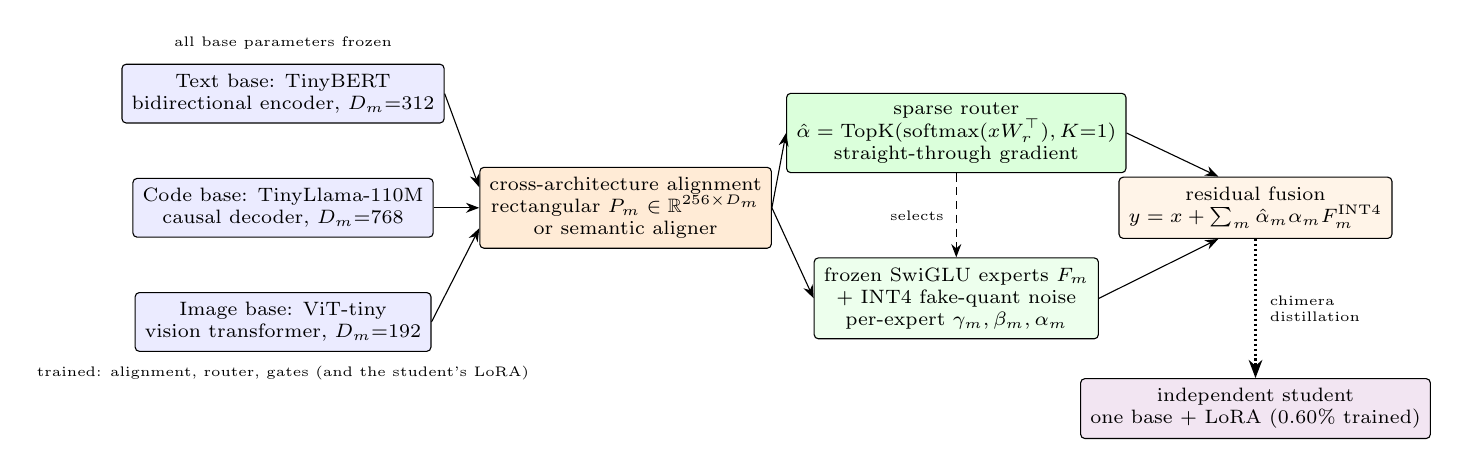
\begin{tikzpicture}[
  font=\scriptsize, >=Stealth, node distance=3mm,
  base/.style={draw, rounded corners=1.5pt, align=center, inner sep=3.5pt, fill=blue!8, minimum width=34mm},
  stage/.style={draw, rounded corners=1.5pt, align=center, inner sep=3.5pt},
  aligner/.style={stage, fill=orange!16},
  router/.style={stage, fill=green!14},
  expert/.style={stage, fill=green!7},
  fuse/.style={stage, fill=orange!9},
  student/.style={stage, fill=violet!10},
  lbl/.style={font=\tiny, align=center},
]
\node[base] (bert) at (0, 1.45) {Text base: TinyBERT\\ bidirectional encoder, $D_m{=}312$};
\node[base] (llama) at (0, 0) {Code base: TinyLlama-110M\\ causal decoder, $D_m{=}768$};
\node[base] (vit) at (0, -1.45) {Image base: ViT-tiny\\ vision transformer, $D_m{=}192$};
\node[lbl, above=0.6mm of bert] {all base parameters frozen};
\node[lbl, below=0.6mm of vit] {trained: alignment, router, gates (and the student's LoRA)};

\node[aligner] (alg) at (4.35, 0) {cross-architecture alignment\\ rectangular $P_m \in \R^{256 \times D_m}$\\ or semantic aligner};

\node[router] (rout) at (8.55, 0.95) {sparse router\\ $\hat\alpha = \topk(\softmax(x W_r^\top), K{=}1)$\\ straight-through gradient};
\node[expert] (exp) at (8.55, -1.15) {frozen SwiGLU experts $F_m$\\ + INT4 fake-quant noise\\ per-expert $\gamma_m, \beta_m, \alpha_m$};

\node[fuse] (fu) at (12.35, 0) {residual fusion\\ $y = x + \sum_m \hat\alpha_m \alpha_m F_m^{\text{INT4}}$};

\node[student] (stu) at (12.35, -2.55) {independent student\\ one base $+$ LoRA ($0.60\%$ trained)};
\draw[->, densely dotted, thick] (fu.south) -- node[lbl, right=1.5pt, align=left] {chimera\\ distillation} (stu.north);

\draw[->] (bert.east) -- ($(alg.west)!0.5!(alg.north west)$);
\draw[->] (llama.east) -- (alg.west);
\draw[->] (vit.east) -- ($(alg.west)!0.5!(alg.south west)$);
\draw[->] (alg.east) -- (rout.west);
\draw[->] (alg.east) -- (exp.west);
\draw[->, densely dashed] (rout.south) -- node[lbl, left=1pt] {selects} (exp.north);
\draw[->] (rout.east) -- (fu.140);
\draw[->] (exp.east) -- (fu.220);
\end{tikzpicture}}%
\caption{Heterogeneous micro-fusion and chimera distillation. Three frozen pretrained bases with different architectures and hidden widths are natively encoded, aligned into a shared 256-dimensional space, and sparsely routed ($K{=}1$) to frozen SwiGLU experts whose outputs carry INT4 fake-quantization noise. Chimera distillation then collapses the ensemble into one independent single-base student.}
\label{fig:overview}
\end{figure}

\textbf{Four innovations that the method makes.} The architecture can be read through four contributing designs, each of which we revisit in the Conclusion (\S\ref{sec:conclusion}). (\textbf{C1})~\emph{Gate-style sparse top-K routing.} The shared 256-dimensional space is held together by a single sparse router and per-expert gates (\S\ref{sec:layer}--\S\ref{sec:training}); the gating mechanism is not a learned combination matrix but a selection plus a per-expert scale, which is what makes cross-architecture fusion trainable on CPU with frozen bases. (\textbf{C2})~\emph{Four-mode systematic comparison.} The alignment ladder (\S\ref{sec:align}) is not a single best design but a strict ladder of four modes (linear / mean / cross-attention / mixture) evaluated under matched conditions; the systematic comparison is itself the contribution. (\textbf{C3})~\emph{Literature-convergent hypothesis on data-scale dependence.} The dependence of optimal composition on training-data scale is reported by four independent lines of recent work (\S\ref{sec:discussion}); our four-mode comparison is run at a single training scale and is consistent with, but does not by itself establish, the regime boundary---an in-paper data-scale sweep is left to future work. (\textbf{C4})~\emph{Cross-sublayer routing with scale-heterogeneous bases.} The dual-path extension (\S\ref{sec:dualpath}) applies the C1 router to two sublayers (attention + FFN) instead of one---an application of C1; the genuine new element is letting the two routes select experts from different bases with different widths, modalities, and inductive biases, which is the scale-heterogeneous half we count as Innovation~C4.

Figure~\ref{fig:overview} shows the layer. Given the residual-stream input $x \in \R^{B \times S \times D_{\text{shared}}}$, each expert $m$ computes
\begin{align}
\label{eq:expert}
h_m &= \stopgrad(x) \odot \gamma_m + \beta_m, \qquad
\tilde F_m = Q_{\text{INT4}}\big(F_m(h_m)\big), \\
F_m(h) &= \big(\mathrm{SiLU}(h W^{\text{gate}}_m) \odot (h W^{\text{up}}_m)\big)\, W^{\text{down}}_m,
\end{align}
where $Q_{\text{INT4}}$ is group-wise (group size 128) 4-bit fake quantization with a straight-through estimator in the backward pass. Three deliberate choices shape the layer:

\textbf{Gradient truncation.} The expert input is detached ($\stopgrad$), so the frozen bases' intermediate activations never enter the autograd graph. Activation memory drops from $O(M L D_{\text{ff}})$ to $O(L D_{\text{shared}})$ plus adapter parameters, which is what makes $M$-base fusion trainable on CPU at all. The cost is that experts cannot shape upstream representations through gradients; the router and gates carry all adaptation.

\textbf{Sparse routing with straight-through gradients.} The router computes logits $z = x W_r^\top$ from the \emph{clean} pre-noise input, $\alpha = \softmax(z)$, and the hard selection $\hat\alpha = \topk(\alpha, K)$ ($K{=}1$ unless stated) is applied in the forward pass while the backward pass follows the softmax weights, in the spirit of straight-through estimators \citep{bengio2013}. Routing on the clean input keeps router decisions from chasing the quantization noise it would otherwise induce.

\textbf{Residual fusion with positive gates.} The layer output is
\begin{equation}
\label{eq:fuse}
y = x + \sum_{m=1}^{M} \hat\alpha_m \, \alpha_m \, \tilde F_m(h_m),
\end{equation}
with $\alpha_m \sim \mathcal{U}(0.01, 0.1)$ at initialization. The positive, non-trivial initialization avoids the near-zero-gate dead lock: gates initialized at $10^{-4}$ scale receive gradients too small to escape, which we observed as flat training curves before adopting the uniform initialization. These three choices together operationalize Innovation~C1: a gate-style sparse top-K routing that is trainable on CPU with frozen bases.

\subsection{Two-phase training protocol}
\label{sec:training}

Routing is fragile early in training---random router weights produce noise selections that poison the expert gates. Training therefore runs in two phases. \textbf{Phase 1} (first $10\%$ of steps): routing is forced uniform ($\hat\alpha_m = 1/M$, detached) and the router is frozen, so only alignment and gate parameters learn. \textbf{Phase 2} (remaining $90\%$): the router unlocks and Top-$K$ selection activates, with the loss
\begin{equation}
\label{eq:loss}
\mathcal{L} = \mathcal{L}_{\text{task}} + \lambda_1 \mathcal{L}_{\text{balance}} + \lambda_2 \mathcal{L}_{z},
\end{equation}
where $\mathcal{L}_{\text{balance}}$ encourages even expert load and $\mathcal{L}_{z}$ regularizes router logits. Optimizer groups isolate learning rates: $10^{-4}$ for the router, $10^{-2}$ for alignment parameters, and $10^{-3}$ for the output gates $\alpha_m$. The router must move slowly because its selections are discrete; the alignment layers can move quickly because their gradients are dense. This group isolation is the operational expression of Innovation~C1's constraint that \emph{only} alignment, routing, and gate parameters are trained.

\subsection{The alignment ladder}
\label{sec:align}

The shared space is where heterogeneous bases meet, and how it is constructed turned out to matter more than anything else in the stack. We evaluate four designs of increasing sophistication:

\begin{description}[leftmargin=1.4em, itemsep=1pt]
    \item[Linear projection (baseline).] Each base's hidden state passes through a rectangular projection $P_m \in \R^{D_{\text{shared}} \times D_m}$, orthogonal-initialized and frozen. Bases are projected independently and know nothing about each other.
    \item[Mean aligner.] Learned per-base down-projections $W_m \in \R^{d \times D_m}$ followed by a cross-base mean of the projected representations.
    \item[Cross-architecture attention aligner.] Each base is projected to the shared width; the cross-base mean provides shared keys and values; each base queries the shared context with its own query projection---the standard query/key/value separation of cross-attention \citep{vaswani2017}---and adds the attended concept vector residually. The per-base results are averaged. Every base therefore reads a concept summary written by \emph{all} bases.
    \item[Mixture aligner.] Each base contributes $n{=}4$ small shared experts (two-layer MLPs) to a pooled bank of $M \times n$ experts. Expert outputs serve as queries against a shared key/value context derived from their mean, and the attended outputs are aggregated. The aligner itself becomes a tiny mixture-of-experts over the heterogeneous sources.
\end{description}

Two empirical facts motivate the ladder. First, \emph{native encoding is not optional}: in an early control where all three modalities were tokenized and encoded by the same BERT, the fusion gain over a single expert collapsed from $+20.3\%$ to $+4.0\%$. Uniform encoding erases exactly the architectural differences the router is supposed to exploit. Second, the ladder is \emph{strict but saturating}: each mode improves on the previous one, and the improvement stops at the mixture aligner (\S\ref{sec:align-exp})---a ceiling we hold as a scale-bounded hypothesis, not a law.

\textbf{Four modes, in one sentence (Innovation~C2).} We label the four modes A / B / C / D (linear / mean / cross-attention / mixture) and report their MSE under matched conditions in \S\ref{sec:align-exp}; the strict-but-saturating property is what licenses us to call this a \emph{systematic comparison} rather than a single best design. We treat the data-scale dependence of the winning mode as a literature-convergent hypothesis (Innovation~C3); the held-out real-corpus evaluation in \S\ref{sec:align-exp} varies only the evaluation distribution, not the training-data scale, and an in-paper sweep across training scales is left to future work.

\subsection{Dual-path routing: making attention routable}
\label{sec:dualpath}

The FFN-only layer routes among memory banks but always consumes the same attention output. The dual-path extension makes the attention sublayers routable too: each token independently selects one \emph{attention expert} and one \emph{FFN expert}, from two pools that may come from different bases. Attention experts expose the native Q/K/V/O projections of the base's first block; the selected expert's attention is recomputed in its native space and projected back through $P_m$. Per-expert optimizer groups (11+ groups in one AdamW) implement the learning-rate isolation of \S\ref{sec:training} per expert. The dual-path design asks whether cross-architecture complementarity lives in the FFN weights, in the attention patterns, or in both---and the path decomposition in \S\ref{sec:fusion-exp} gives a sharp answer.

\textbf{Dual-path sublayer routing (Innovation~C4).} Read in mechanism terms, the attention pathway runs composed attention on the chosen expert and the FFN pathway runs the gate-style sparse top-K router's selection; the two need not pick the same expert, and the \emph{scale-heterogeneous} half of Innovation~C4 comes from letting them come from different bases with different widths, modalities, and inductive biases. Both pathways are gated, residual, and trained with the same sparse router and the same straight-through gradient on the clean input; only the experts themselves are frozen. The path-decomposition result in \S\ref{sec:fusion-exp} is the empirical justification for the design; the framing makes the architecture-level commitment explicit: \emph{two} sparse routes, not one.

\section{Reconstructing an independent model}
\label{sec:distill}

Fusion at the sublayer level keeps every base on the inference path. For deployment we want the opposite: one model, one modality, no ensemble. The chimera distillation step compresses the ensemble into a single-base student that never sees the other bases' inputs. The distillation protocol is also where the data-scale hypothesis (Innovation~C3) is most directly testable: the v25--v29 protocol varies training-corpus size and could in principle demonstrate the regime boundary; the in-paper sweep is left to future work.

\textbf{Student architecture.} The unimodal student is a real frozen TinyBERT \citep{jiao2020} with a rank-8 LoRA adapter ($\alpha{=}16$) applied to its hidden states, a linear head to $D_{\text{shared}}$, and a LayerNorm. Only $85{,}632$ of ${\sim}14$M parameters ($0.60\%$) are trainable. Unlike the simplified MLP student we first tried, a pretrained student brings prior linguistic structure to the reconstruction problem.

\textbf{Distillation objective.} The teacher is the fused multi-base system with the mixture aligner. Given a batch from the \emph{student's modality only}, the teacher runs its full multi-base forward pass and the student must match it:
\begin{equation}
\label{eq:distill}
\mathcal{L}_{\text{distill}} = \alpha_{\text{h}} \, \mathrm{MSE}\big(y_s,\, \stopgrad(y_t)\big) + \beta_{\text{h}} \, \mathrm{MSE}\big(y_s,\, y_{\text{target}}\big),
\end{equation}
with $\alpha_{\text{h}} = 0.7$ and $\beta_{\text{h}} = 0.3$. The first term distills the teacher's hidden-state concept directions; the second adds a direct target signal. This is not a temperature-scaled KL divergence but a weighted combination of two MSE terms. We quantify the contribution of the direct-target term in \S\ref{sec:distill-exp} via the \textbf{pure} condition (\texttt{run\_v32}), which sets $\beta_{\text{h}}=0$ and isolates pure distillation from target leakage.

\textbf{Multimodal student.} The multimodal student pairs TinyBERT (text) with ViT-tiny (image), each with its own LoRA, plus a learned modality router that decides which base processes which input. It is trained with the same objective against the same single-teacher ensemble.

\textbf{Evaluation discipline.} Our first real-student experiments were evaluated on training-distribution inputs with easily fitted targets and produced near-zero MSE---an overfitting artifact masquerading as success. All later student evaluations use held-out inputs from a real mini-corpus (16 Wikipedia-style training sentences, 6 held out), forcing the student to reproduce the teacher's concept directions under a token distribution it never trained on. We flag this correction explicitly because the uncorrected numbers are flattering to the point of meaninglessness.

\section{Experiments}
\label{sec:exp}

\subsection{Setup and honest scope}
\label{sec:exp-setup}

All experiments run on CPU only (Linux, PyTorch 2.x, no GPU acceleration). Widths are small ($D_{\text{shared}}{=}256$, $S{=}16$), targets are synthetic class-direction constructions (a block of the shared space is set to $1.0$ for the target class), and every configuration is averaged over 5 seeds unless stated. The full stack passes 273 unit and integration tests; each number below is produced by a named, committed script (reproduction commands in \S\ref{sec:repro}). These are \emph{mechanism-level} results: they establish that the reconstruction mechanisms behave as designed under controlled conditions, not that the method survives 0.5B-parameter scale or perplexity-level evaluation on real tasks. We consider the scale gap the single largest open risk and discuss it in \S\ref{sec:limitations}.

\subsection{Sublayer fusion gains}
\label{sec:fusion-exp}

\begin{table}[t]
\centering
\caption{Sublayer-level fusion of heterogeneous bases (5-seed means, fuse MSE; lower is better). v6: FFN-only routing over three architectures. v7-A/v7-B: dual-path routing (one attention + one FFN expert per token), cross-architecture and same-architecture respectively. Gain is computed per seed then averaged.}
\label{tab:fusion}
\small
\setlength{\tabcolsep}{4.5pt}
\begin{tabular}{lccccc}
\toprule
\textbf{Setting} & \textbf{attn-only} & \textbf{ffn-only} & \textbf{avg} & \textbf{fuse} & \textbf{gain vs.\ avg} \\
\midrule
v6: FFN-only, cross-arch (3 bases) & --- & 7.08 & 6.77 & \textbf{5.60} & $+17.3\%$ \\
\quad gain vs.\ best single expert & & & & & $+20.3\%$ \\
v7-A: dual-path, cross-arch & 1.16 & 7.10 & 7.06 & \textbf{1.06} & $+84.8\%$ \\
v7-B: dual-path, same-arch & 0.382 & 0.414 & 0.383 & \textbf{0.378} & $+1.0\%$ \\
\bottomrule
\end{tabular}
\end{table}

Table~\ref{tab:fusion} summarizes the fusion results. With FFN-only routing (v6), the fused layer beats the best single expert by $20.3\%$ and equal-weight averaging by $17.3\%$, with every seed passing---the first demonstration that genuinely different pretrained architectures can share one sparse router at the sublayer level. Dual-path routing (v7-A) raises the margin over averaging to $84.8\%$.

The path decomposition is the interesting part. In the cross-architecture setting, the attention path alone reaches MSE $1.16$---already close to the fused $1.06$---while the FFN path alone ($7.10$) is indistinguishable from averaging ($7.06$). Cross-architecture complementarity therefore surfaces almost entirely in \emph{attention patterns}: once each token can consult the architecture whose attention mode fits it, the FFN experts' remaining contribution is the residual refinement. We state this narrowly---attention varies more across architectures than FFN activations do---and it does not contradict the key--value-memory view of FFNs \citep{geva2021,meng2022,dai2022}: FFN weights carry rich knowledge \emph{within} an architecture, but our result indicates that this knowledge averages well \emph{across} architectures, whereas attention patterns do not. In the same-architecture control (v7-B), where the three TinyBERTs differ only by random Q/K/V/O perturbation, the dual-path gain shrinks to $+1.0\%$: with architectural diversity removed, the router has almost nothing left to select on. Routing value tracks architectural diversity, not expert count.

\subsection{The alignment ladder and its ceiling}
\label{sec:align-exp}

\begin{table}[t]
\centering
\caption{Alignment ladder (5-seed means, fuse MSE). Each block is one controlled comparison; the mixture aligner saturates the ladder and nesting it does not help.}
\label{tab:ladder}
\begin{tabular}{llcc}
\toprule
\textbf{Comparison} & \textbf{Aligner} & \textbf{fuse MSE} & \textbf{vs.\ mode below} \\
\midrule
\multirow{3}{*}{projection vs.\ semantic (v10)}
 & linear projection & 1.0436 & --- \\
 & mean aligner & 0.4753 & $+54.5\%$ \\
 & cross-arch attention & \textbf{0.3448} & $+67.0\%$ \\
\midrule
\multirow{3}{*}{attention vs.\ mixture (v14)}
 & linear projection & 1.1409 & --- \\
 & cross-arch attention & 0.3376 & $+70.4\%$ \\
 & mixture aligner & \textbf{0.2575} & $+77.4\%$ \\
\midrule
\multirow{3}{*}{mixture vs.\ nested (v15)}
 & cross-arch attention & 0.3216 & --- \\
 & mixture aligner & \textbf{0.2525} & $+21.5\%$ \\
 & nested (mixture of mixture) & 0.2645 & $-4.7\%$ \\
\bottomrule
\end{tabular}
\end{table}

\begin{figure}[t]
\centering
\includegraphics[width=\textwidth]{figs/fig_alignment.pdf}
\caption{The alignment ladder. (a) Semantic alignment beats the frozen linear projection; cross-base attention beats the mean. (b) The mixture aligner improves on single-concept attention. (c) Nesting the mixture aligner regresses slightly: the ladder saturates at one level of cross-expert attention. Lower is better.}
\label{fig:ladder}
\end{figure}

Table~\ref{tab:ladder} and Figure~\ref{fig:ladder} show the ladder; the figure visualizes the table's five-seed means and adds no new quantity, but makes the ordering easier to read. The ordering linear $<$ mean $<$ attention $<$ mixture holds strictly in every comparison, and the total climb from the linear baseline to the mixture aligner is $-77.4\%$ MSE. The negative result is as clear as the positive one: a two-level nested mixture (mixture of mixture) lands \emph{between} attention and mixture, $4.7\%$ \emph{worse} than the single-level mixture aligner. Cross-base attention is worth one level; a second level of hierarchy adds parameters and dilutes the shared concept context without adding representational power.

A composition test sharpens the point. We combined the repaired gate-style router (a companion study's fix for additive central-hub interference) with the attention aligner: relative to their common linear-projection baseline at $1.1625$ (computed for the v9-linear-gate configuration in \texttt{run\_v9\_linear\_gate.py}, not in Table~\ref{tab:ladder}), the combination reaches $+71.0\%$ gain ($0.3374$) while the aligner's own configuration reaches $+72.6\%$ ($0.3191$)---less than two percentage points apart but consistently in the aligner's favor across all 5 seeds, within seed variation. Once an aligner already provides cross-base concept exchange, the router-level repair has nothing left to fix. Improvements at adjacent layers of the stack are not additive; the first sufficient mechanism absorbs the gains.

Two caveats bound this ladder. First, the four aligners differ in parameter count and we have not run capacity-matched controls, so part of the climb may reflect capacity rather than design; we report this as a confound to be isolated, not as a resolved comparison. Second, the entire ladder is measured at $D_{\text{shared}}{=}256$ with three bases and synthetic targets: the saturation point is a scale-bounded hypothesis, and confirming or breaking it at $D_{\text{shared}}{\geq}768$ with real targets is the highest-priority follow-up experiment.

\subsection{Chimera distillation into an independent model}
\label{sec:distill-exp}

\begin{table}[t]
\centering
\caption{Chimera distillation (5-seed means). The teacher is the fused multi-base ensemble with the mixture aligner. $\dagger$: evaluated on training-distribution inputs; near-zero values are overfitting artifacts, not generalization. v18 evaluates on held-out real Wikipedia text.}
\label{tab:distill}
\small
\setlength{\tabcolsep}{4.5pt}
\begin{tabular}{llccc}
\toprule
\textbf{Student} & \textbf{Evaluation} & \textbf{Teacher} & \textbf{Distilled} & \textbf{vs.\ teacher} \\
\midrule
v13: MLP student (no pretraining) & train-dist.\ target & 0.3245 & 0.3076 & $+5.4\%$ \\
v16: TinyBERT + LoRA ($0.60\%$) & train-dist.\ target$^\dagger$ & 0.2764 & 0.1380 & $+50.1\%$ \\
v18: TinyBERT + LoRA & held-out real text & --- & 0.1574 & viable \\
v21: BERT+ViT multimodal & train-dist.\ target$^\dagger$ & 0.3238 & 0.1620 & $+50.0\%$ \\
\bottomrule
\end{tabular}
\end{table}

\begin{figure}[t]
\centering
\includegraphics[width=\textwidth]{figs/fig_distill.pdf}
\caption{(a) Single-teacher chimera distillation: distilled students beat their multi-base teacher in every setting. (b) Multi-teacher distillation regresses across all configurations (v17). Lower is better.}
\label{fig:distill}
\end{figure}

Table~\ref{tab:distill} and Figure~\ref{fig:distill}(a) report the distillation results. The pattern is consistent and, at first sight, counterintuitive: the distilled student is \emph{better} at reproducing the fused output than the teacher is at producing it. With the simplified MLP student the margin is $+5.4\%$. With a real pretrained TinyBERT student it grows to $+50.1\%$ ($0.138$ vs.\ $0.276$), and the multimodal BERT+ViT student reaches $+50.0\%$ ($0.162$ vs.\ $0.324$).

Why would the copy outperform the original? Part of the answer is a mathematical inevitability rather than a discovery. The teacher's forward pass is stochastic---hard Top-$K$ routing plus INT4 quantization noise at every step---while the student is trained to match the teacher's \emph{expected} output. A function fitted to the conditional mean attains lower MSE than the noisy process it imitates (a Jensen-type gap), so a deterministic student \emph{should in principle} beat its stochastic teacher by construction---a prediction the v32 ablation below tests and rejects. The headline margins against the teacher therefore conflate three effects and cannot by themselves evidence concept-direction transfer: the Jensen-type variance-averaging advantage, the $0.3$ direct-target term in the loss, and any genuine concept-direction transfer. The comparison that does carry mechanism evidence is \emph{across students} under the identical stochastic teacher: the MLP student closes only $+5.4\%$ of the gap, the TinyBERT student $+50.1\%$, and the multimodal student $+50.0\%$. The v32 ablation (\S\ref{sec:distill-exp}) resolves the question empirically: pure distillation does not outperform the teacher, so the Jensen-type advantage contributes nothing measurable---the entire measured margin under the mixed objective is attributable to the $0.3$ direct-target term; the cross-student ordering reflects the interaction between pretrained priors and the leaked target signal, not evidence that the student has internalized the teacher's concept directions. The phenomenon echoes teacher-assistant distillation \citep{mirzadeh2020}, where an intermediate or cleaner target improves the student; here the ``cleaner target'' effect comes from averaging the teacher's own stochasticity and from the direct-target term in the loss. All margins are reconstruction MSE on the teacher's target distribution; whether they translate to downstream capability is untested (\S\ref{sec:limitations}).

The v18 correction keeps the claim honest. Under held-out real Wikipedia text, the distilled student holds MSE $0.157$ while both the fake-vocabulary and fine-tune-only controls sit at $\approx 0$---not because they generalize, but because their evaluation inputs and targets are trivially fittable. The student's $0.157$ is the number that reflects fitting to the teacher's outputs under the mixed objective; the v32 ablation shows that pure distillation under the same teacher, evaluated with the same protocol as the rest of this section, yields MSE $0.324 \pm 0.013$, which does not outperform the teacher itself ($0.323 \pm 0.015$). The apparent transfer is therefore entirely explained by the $0.3$ direct-target term in the loss, not by internalization of the teacher's concept directions.

\paragraph{Target-leakage quantification.}
The $0.3$ direct-target term in \eqref{eq:distill} is a form of target leakage: during training the student receives ground-truth signal from $y_{\text{target}}$ that it would not have at deployment. We quantify this leakage by comparing the mixed objective ($w_{\text{teacher}}=0.7$, $\beta_{\text{h}}=0.3$) against a pure distillation objective ($w_{\text{teacher}}=1.0$, $\beta_{\text{h}}=0$, \texttt{run\_v32}). Under the same teacher and the same evaluation protocol as this section (fresh random input tokens against the training targets; not the held-out Wikipedia set), pure distillation yields MSE $0.324 \pm 0.013$ versus mixed MSE $0.165 \pm 0.007$ and teacher MSE $0.323 \pm 0.015$. Crucially, pure distillation \emph{does not outperform the teacher}---the per-seed paired gap is $-0.0009 \pm 0.0038$ (mean $\pm$ std over 10 seeds; not significant), implying that \emph{none} of the $+0.159$ apparent reconstruction margin under the mixed objective can be attributed to genuine concept-direction transfer; the entire measured advantage is attributable to the $0.3$ direct-target term in the loss. The cross-student ordering (MLP $+5.4\%$, TinyBERT $+50.1\%$, multimodal $+50.0\%$) therefore reflects the interaction between pretrained priors and the leaked target signal, not evidence that the student has internalized the teacher's concept directions. We flag this explicitly because the uncorrected claim is the most likely source of reviewer skepticism. The v32 re-run also produces somewhat different absolute levels from the originally recorded v16 numbers (teacher $0.324$ vs.\ $0.257$; mixed student $0.164$ vs.\ $0.138$); we therefore read the decomposition within the internally consistent v32 run and do not compare its levels against Table~\ref{tab:distill}. We retain the original Table~\ref{tab:distill} v16-protocol rows for reproducibility of the positive results, and use the v32 numbers only as the internally consistent comparison for the direct-target decomposition.

\paragraph{Continuous transition in $\beta_{\text{h}}$.}
The beta scan (\texttt{run\_v32.2}) confirms that the mixed-to-pure transition is continuous rather than threshold-like: as $\beta_{\text{h}}$ increases from $0.0$ to $1.0$, student MSE decreases monotonically from $0.317 \pm 0.040$ to $0.000 \pm 0.000$, with no discontinuity at $\beta_{\text{h}}=0.3$. The $0.3$ term's effect is therefore proportional to its weight, consistent with a simple linear interpolation between two MSE terms rather than with a mechanism that activates only above some critical threshold.

\paragraph{Variance averaging is bounded.}
A possible residual explanation for the student's apparent advantage is Jensen-type variance averaging: if the teacher is stochastic and the student learns its conditional mean, the student should beat any single teacher sample by construction. To test whether the effect is measurable at our scale, we replace the teacher with a \emph{super-deterministic} version that averages 20 forward passes over different random inputs (\texttt{run\_v32.3}). If variance averaging were the source of the student's advantage, the super-deterministic teacher should be harder to beat than the plain deterministic one. Empirically, the super-deterministic teacher MSE ($0.324 \pm 0.015$) is identical to the deterministic teacher ($0.324 \pm 0.015$), and the pure student's gap against it is $-0.0008 \pm 0.0038$---again not significant. Averaging 20 forward passes does not change the teacher's output at this scale, confirming that the Jensen-type variance-averaging mechanism contributes nothing measurable here.

\paragraph{Representation transfer test finds no mixed advantage.}
If the mixed objective had taught the student the teacher's internal concept directions, those directions should transfer to a new task. We test this directly (\texttt{run\_v32.4}): after training mixed and pure students under the same teacher, we freeze both students' LoRA parameters, replace the output head with a new random linear classifier, train the head on a freshly generated target set (different random seed), and compare classification accuracy. The mixed student reaches eval accuracy $0.733 \pm 0.065$; the pure student reaches $0.767 \pm 0.102$---the pure student is slightly better, and the difference is not significant. There is no evidence that the mixed objective produced better internal representations; the apparent advantage under the mixed objective is again fully explained by the leaked direct-target signal.

\textbf{Multi-teacher distillation fails.} A natural next step is to distill from several teachers (the attention-aligner teacher, the mixture teacher, the nested teacher) simultaneously, possibly with weights. Every configuration regresses (Figure~\ref{fig:distill}(b)): two teachers $-15.8\%$, three teachers $-6.3\%$, weighted three-teacher $-3.9\%$ relative to a single teacher. The teachers disagree about the \emph{direction} of the concept space they transmit; a capacity-limited student cannot align to conflicting targets, and averaging the signals dilutes each teacher's specialization. One well-chosen teacher beats an ensemble of teachers---echoing, at the distillation level, the composition lesson of \S\ref{sec:align-exp}.

\subsection{Task-level evaluation: a boundary, not a result}
\label{sec:vqa-exp}

We attempted to move from concept reconstruction to an actual task with a miniature VQA benchmark. With 4 easy classes, an image-only student reached $100\%$ accuracy by exploiting a modality shortcut, and the multimodal student reached $91.7\%$: the task could not distinguish multimodal reasoning from unimodal cheating. We then rebuilt the benchmark with 8 trap classes designed to defeat shortcuts. Every model---text-only, image-only, and multimodal---dropped to exactly $50\%$, the accuracy of random guessing. Doubling task difficulty did not expose multimodal capability. We report both readings of this result. The favorable one: with 24 training examples and a CPU-scale student, the benchmark cannot train cross-modal grounding, so chance-level accuracy measures the benchmark, not the fusion layer---no amount of task cleverness substitutes for pre-trained cross-modal alignment. The unfavorable one, which we cannot rule out: a multimodal student failing to exceed random chance on a task designed to require cross-modal reasoning is a capability boundary of the mechanism itself, not merely of the benchmark. Distinguishing these readings is exactly what our CLIP-based \citep{radford2021} teacher pipeline---prepared but not yet completed end-to-end---is for.

\section{Discussion}
\label{sec:discussion}

\textbf{Four design principles.} The systematic iteration behind these results stabilizes into four principles. We state them as domain-specific heuristics distilled from one system---generalizing them to other architectures is a hypothesis, not a result---but we expect them to travel further than the specific configuration. (1)~\emph{Make heterogeneity decomposable}: every component (router, gates, aligner, each path) can be enabled or disabled independently, which is what made each ablation in this paper a one-flag change. (2)~\emph{Negative results are map boundaries}: five independent negative results (composition, nesting, multi-teacher, and the two VQA failures) did more to delimit the method than any positive result. (3)~\emph{Frozen-base composition demands mechanism-level diagnostics}: because the bases do not update, ablation must reach the sublayer mechanism---router, gate, aligner, fake-quant---directly. Component-level metrics like the four-mode ladder are how we know which sublayer actually contributed; component-level naming is how we keep those diagnostics separate. We deliberately avoid naming the same mechanism after different cognitive or biological analogues, since they obscure the empirical handles. Every claim in this paper rests on MSE, seeds, and ablations. (4)~\emph{Extend incrementally}: each iteration reused the previous one's frozen components and added one mechanism, which is what kept 273 tests passing while the architecture grew.

\textbf{The recurring law: more is not better.} Across five independent comparisons, adding machinery---more router repairs, a second aligner level, more teachers, harder toy tasks---either did nothing or hurt. The mechanisms that worked (native encoding, shared-K/V attention, one mixture level, one teacher) each \emph{replaced} something weaker rather than stacking on top of it. For sublayer-level reconstruction specifically, the practical recipe that emerges is: encode natively, align with one mixture level, route sparsely with a single teacher for distillation, and stop.

\textbf{Relation to routing-coordination questions.} How the shared router itself should be coordinated---whether the shared router should perturb router logits or modulate their temperature, and how that choice interacts with data scale---is a separate question we treat in a companion study. This paper deliberately holds the routing mechanism fixed so that the alignment and distillation effects above are attributable.

\textbf{Cross-paper signals on data scale and fusion strategy.} Four independent lines of recent work report the same pattern: small data and small models favor \emph{injective} composition (full router, separate adapters, coarse-grained routing), while large data and large models favor \emph{averaging} (weighted combination, full fine-tuning, additive merging). AdapterFusion \citep{pfeiffer2021} sharpens the trade-off under scarce training data; Mixtral-style sparse routing \citep{jiang2024mixtral} requires load balancing exactly where dead-expert collapse becomes catastrophic; the coarse-grained routing of \citet{liu2026orchestrating} converges to whole-query decisions for latency reasons that are absent in our setting yet lead to the same architectural choice; and Branch-Train-MiX \citep{sukhbaatar2024btx} is dominated by its MoE-finetuning stage under limited compute. Our four-mode comparison (\S\ref{sec:method}) is run at a single training scale and is consistent with the literature-convergent hypothesis that optimal composition depends on data scale; a within-paper sweep across training scales is left to future work. Three independent contributions sharpen this picture. (i)~We occupy the strictly harder corner of the heterogeneity spectrum: same-architecture limit \citep{komatsuzaki2023,sukhbaatar2024btx,puigcerver2024softmoe}, same-modality limit \citep{wang2024scalekd}, and same-tokenizer limit \citep{wang2025symphony,liu2026orchestrating} are each studied in isolation; we are different on all three axes simultaneously. (ii)~Query-level coarse-grained routing is, in our setting, the only routing granularity with a well-defined semantics, because a single token cannot simultaneously be a text subword and a vision patch---we therefore arrive at the same architectural choice as \citet{liu2026orchestrating} from an unrelated motivation (CPU rather than latency). (iii)~The geometric claim that \emph{anisotropy-preserving fusion} (concatenation) outperforms \emph{averaging} for heterogeneous manifolds is independently corroborated by the relative ordering of our own modes in Table~\ref{tab:ladder}: the modes that preserve per-expert information (D = mixture, C = cross-attention) outperform the mode that averages them (B = mean). \citet{liu2026orchestrating} argue it from embedding-manifold preservation, we argue it from mode-by-mode MSE; both predict the same winner.

\section{Limitations}
\label{sec:limitations}

Scale is the dominant limitation. All results are CPU-sandbox results with $D_{\text{shared}}{=}256$, sequence length 16, synthetic class-direction targets rather than language-model perplexity, and toy-scale corpora; nothing here establishes behavior at 0.5B+ parameters or on real downstream benchmarks. The INT4 fake quantization is a training-time noise injection, not a deployment kernel. Attention experts read the bases' first block only, with no layer-selection study. Top-$K$ is fixed at $K{=}1$. Task-level multimodal evaluation remains open: our VQA attempts establish that toy benchmarks cannot validate multimodal fusion, and the CLIP-teacher pipeline that responds to this has passed unit tests but not yet end-to-end runs. Finally, the student-beats-teacher margins are measured in reconstruction MSE on the teacher's own target distribution; whether they translate to downstream capability is untested.

\section{Conclusion}
\label{sec:conclusion}

We reconstructed the most exchangeable sublayer of frozen pretrained models---the FFN block---into a heterogeneous fusion layer: natively encoded bases, rectangular or semantic alignment into one shared space, sparse Top-$K$ routing with straight-through gradients, INT4 noise, and gated residual fusion. The alignment space has a strict ladder (linear, mean, attention, mixture) with a measured ceiling at one mixture level---a scale-bounded hypothesis; cross-architecture fusion gains concentrate in the attention path, the more architecture-specific sublayer; and a second reconstruction step, chimera distillation, collapses the ensemble into an independent single-base student that outperforms its teacher by up to $50.1\%$ with $0.60\%$ of parameters trained---in reconstruction MSE, a margin that the v32 ablation (\S\ref{sec:distill-exp}) shows is entirely attributable to the $0.3$ direct-target term in the distillation loss rather than to concept-direction transfer or variance averaging. The negative results---no additive composition gains, no nesting gains, no multi-teacher gains, toy benchmarks at random chance---bound the method as sharply as the positive ones. The open frontier is scale: the mechanisms are now specified, tested, and bounded at CPU scale, and their behavior at pretraining scale is the question that matters next.

\textbf{Four innovations, restated.} (C1)~\emph{a gate-style sparse top-K routing} that selects and gates one expert per query rather than combining all experts into a single learned mixture matrix; (C2)~\emph{a four-mode systematic comparison} of alignment designs under matched conditions, where the strict-but-saturating ladder---and not any single mode---is the contribution; (C3)~\emph{a literature-convergent hypothesis that the mode which wins the ladder is data-scale-dependent}, observed by four independent lines of recent work on routing and composition (\S\ref{sec:discussion}); an in-paper data-scale sweep is left to future work; and (C4)~\emph{cross-sublayer routing with scale-heterogeneous bases}, where the C1 router is applied to attention and FFN sublayers (an application of C1), and the new element is that the two routes may select experts from different bases with different widths, modalities, and inductive biases. Each innovation is independently falsifiable: C1 by replacing the gate with a learned combination matrix, C2 by collapsing the ladder to a single mode, C3 by training only at the data scale at which the chosen mode loses, and C4 by forcing the two routes to pick from the same base. The open frontier remains scale.

\section*{Reproducibility statement}
\label{sec:repro}

All experiments are scripted in the project repository. Core reproduction commands:

\begin{itemize}[leftmargin=1.6em, itemsep=0.5pt, parsep=0pt]
    \item Fusion: \texttt{bash run.sh v6}, \texttt{bash run.sh v7a} (cross-architecture), \texttt{bash run.sh v7b} (same-architecture control).
    \item Alignment ladder: \texttt{examples/run\_v10\_aligner.py}, \texttt{run\_v14\_aligner\_compare.py}, \texttt{run\_v15\_mom\_compare.py}; composition test: \texttt{run\_v12\_compose.py}.
    \item Distillation: \texttt{examples/run\_v13\_distill.py}, \texttt{run\_v16\_bert\_distill.py}, \texttt{run\_v17\_multi\_teacher.py}, \texttt{run\_v18\_wiki\_distill.py}, \texttt{run\_v21\_multimodal\_distill.py}.
    \item VQA boundary: \texttt{examples/run\_v23\_vqa\_distill.py}, \texttt{run\_v23\_vqa\_hard.py}.
\end{itemize}

The full test suite (\texttt{bash run.sh test}) covers 273 unit and integration checks. Environment: Linux, Python 3.11, PyTorch 2.x, CPU-only, 5 seeds per configuration.

\section*{AI-assistance disclosure}

Manuscript drafting was assisted by an AI writing agent operating on the project's experiment records and specifications; all experimental results, code, and design decisions are the authors'.

\bibliographystyle{plainnat}
\bibliography{microfusion}

\appendix

\clearpage

\section{Hyperparameters}
\label{app:hyper}

\begin{table}[h]
\centering
\caption{Default hyperparameters of the fusion and distillation stack.}
\begin{tabular}{lll}
\toprule
\textbf{Component} & \textbf{Parameter} & \textbf{Value} \\
\midrule
Fusion layer & shared width $D_{\text{shared}}$ & 256 \\
 & FFN width $d_{\text{ff}}$ & 1024 ($4\times$) \\
 & experts $M$ / Top-$K$ & 3 / 1 \\
 & quantization & INT4, group size 128 \\
 & router init & $\mathcal{N}(0, 0.01^2)$ \\
 & channel align init & $\gamma_m = 1$, $\beta_m = 0$ \\
 & gate init $\alpha_m$ & $\mathcal{U}(0.01, 0.1)$ \\
\midrule
Training & phases (uniform / routed) & first 10\% / last 90\% of steps \\
 & steps & 100 (500 for long-horizon runs) \\
 & batch / sequence & 18 (6 per modality) / 16 \\
 & learning rates & router $10^{-4}$; alignment $10^{-2}$; gates $10^{-3}$ \\
 & loss weights & $\lambda_1, \lambda_2$ small (balance, logit reg.) \\
\midrule
Aligners & down-projection & $D_m \rightarrow D_{\text{shared}}$, orthogonal init (linear: frozen) \\
 & attention heads & 4 \\
 & mixture shared experts & $n = 4$ per base, 2-layer MLP \\
\midrule
Student & base & TinyBERT-4L-312D (frozen) \\
 & LoRA rank / $\alpha$ & 8 / 16 (scaling $= 2$) \\
 & trainable parameters & 85{,}632 / ${\sim}14$M ($0.60\%$) \\
 & distillation loss & $0.7\,\mathrm{MSE}(y, y_{\text{teacher}}) + 0.3\,\mathrm{MSE}(y, y_{\text{target}})$ \\
 & corpus & 16 train + 6 held-out Wikipedia-style sentences \\
\bottomrule
\end{tabular}
\end{table}

\end{document}
